\documentclass[a4paper]{article} % Create new a report
\usepackage[utf8]{inputenc}
\usepackage[T5]{fontenc} % To use unicode
\usepackage{mathptmx} % Time New Roman
\usepackage[right=2cm,left=3cm,top=2cm,bottom=2.5cm]{geometry}
\usepackage[fontsize=13pt]{scrextend}
\usepackage{graphicx} % Required for inserting images
\usepackage{indentfirst}
\usepackage{float} % Set position of image.
\usepackage{tikz} % Create border
\usepackage{multicol}
\usepackage{caption}
\usepackage{array} % Required for Table Column Text Alignment with Custom Widths
\usepackage{titlesec} % Set font style
\usepackage{parskip}

\usetikzlibrary{calc}
\renewcommand{\baselinestretch}{1.2}
\setlength{\parskip}{6pt} % Spacing after
\setlength{\parindent}{1cm}


\setcounter{secnumdepth}{4} % Heading
\titlespacing*{\section}{0pt}{0pt}{12pt} % Heading 1
\titleformat*{\section}{\fontsize{16pt}{0pt}\selectfont \bfseries}

\titlespacing*{\subsection}{0pt}{10pt}{0pt} % Heading 2
\titleformat*{\subsection}{\fontsize{14pt}{0pt}\selectfont \bfseries }

\titlespacing*{\subsubsection}{0pt}{10pt}{0pt} % Heading 3
\titleformat*{\subsubsection}{\fontsize{13pt}{0pt}\selectfont \bfseries \itshape}

\titlespacing*{\paragraph}{0pt}{10pt}{0pt} % Heading 4
\titleformat*{\paragraph}{\fontsize{13pt}{0pt}\selectfont \itshape}


\renewcommand{\figurename}{\fontsize{12pt}{0pt}\selectfont \bfseries Hình}
\renewcommand{\thefigure}{\arabic{figure}}
% \captionsetup[figure]{labelsep=space}

\renewcommand{\tablename}{\fontsize{12pt}{0pt}\selectfont \bfseries Bảng}
\renewcommand{\thetable}{\arabic{table}}
% \captionsetup[table]{labelsep=space}

\usepackage{lipsum}
\renewcommand{\contentsname}{MỤC LỤC}
\renewcommand{\listfigurename}{DANH MỤC HÌNH}
\renewcommand{\refname}{TÀI LIỆU THAM KHẢO}

\usepackage[unicode]{hyperref}
\usepackage{colortbl}
\definecolor{LightCyan}{rgb}{0.88,1,1}
\usepackage{forloop}
\newcounter{loopcntr}
\newcommand{\rpt}[2][1]{\forloop{loopcntr}{0}{\value{loopcntr}<#1}{#2}}


\newcommand{\setsection}[1]{\section*{#1}\addcontentsline{toc}{section}{#1}}
\newcommand{\setsubsection}[1]{\subsection*{#1}\addcontentsline{toc}{subsection}{#1}}

\newcommand{\myref}[1]{\textbf{\hyperref[#1]{Hình~\ref*{#1}}}}


\begin{document}

\begin{titlepage}
  \begin{tikzpicture}[overlay, remember picture]
    \draw [line width=3pt]
    ($ (current page.north west) + (3.0cm,-2.0cm) $)
    rectangle
    ($ (current page.south east) + (-2.0cm,2.5cm) $);
    \draw [line width=0.5pt]
    ($ (current page.north west) + (3.1cm,-2.1cm) $)
    rectangle
    ($ (current page.south east) + (-2.1cm,2.6cm) $);
  \end{tikzpicture}
  \begin{center}
    \vspace{-6pt}TRƯỜNG ĐẠI HỌC CẦN THƠ \\
    \textbf{\fontsize{16pt}{0pt}\selectfont TRƯỜNG CÔNG NGHỆ THÔNG TIN VÀ TRUYỀN THÔNG}
    % \vspace{0.5cm}
    \begin{figure}[H]
      \centering
      
\includegraphics[width=5cm]{imgs/logo-ctu.png}
    \end{figure}
    \textbf{QUẢN TRỊ HỆ THỐNG} \\
    \textbf{Mã Học Phần: CT179} \\
    \textbf{Nhóm học phần: 04} \\
    \vspace{3.5cm}
    \textbf{\fontsize{16pt}{0pt}\selectfont BÁO CÁO} \\
    \textbf{\fontsize{18pt}{0pt}\selectfont BÀI TẬP TỔNG HỢP CUỐI KỲ} \\
    \vspace{4.5cm}
    \newcommand{\MyIndent}{\hspace{1cm}}
    \begin{tabular}{p{8cm} l}
      \textbf{Giáo viên hướng dẫn}       & \textbf{Sinh viên thực hiện}  \\
      \MyIndent ThS.GV Lê Huỳnh Quốc Bảo & \MyIndent Tên: Trần Thái Toàn \\
                                         & \MyIndent MSSV: B2203534
    \end{tabular}


    \vspace{2cm}
    \fontsize{14pt}{0pt}\selectfont Học Kỳ II, 2023 - 2024
  \end{center}
\end{titlepage}
\cleardoublepage


% Generate menu
\addtocontents{toc}{\protect\thispagestyle{empty}}
\tableofcontents
\thispagestyle{empty}
\cleardoublepage

\pagenumbering{roman}
% \section*{DANH MỤC HÌNH}
% \addcontentsline{toc}{section}{\numberline{}DANH MỤC HÌNH}
% \cleardoublepage

% Automatically generate list figures
\phantomsection
{
  \let\oldnumberline\numberline
  \renewcommand{\numberline}{\figurename~\oldnumberline}
  \listoffigures
}
\addcontentsline{toc}{section}{\numberline{}DANH MỤC HÌNH}
\cleardoublepage


\section*{Mô tả bài tập}

Công ty Tam Quốc chuyên kinh doanh buffet lẩu cay Tứ Xuyên có nhu cầu cài đặt
các dịch vụ mạng phục vụ cho công việc của công ty như sau:

\setcounter{section}{0}
\setcounter{subsection}{1}
\setcounter{figure}{0}
\begin{minipage}{.93\linewidth}
  \captionsetup{type=figure}
  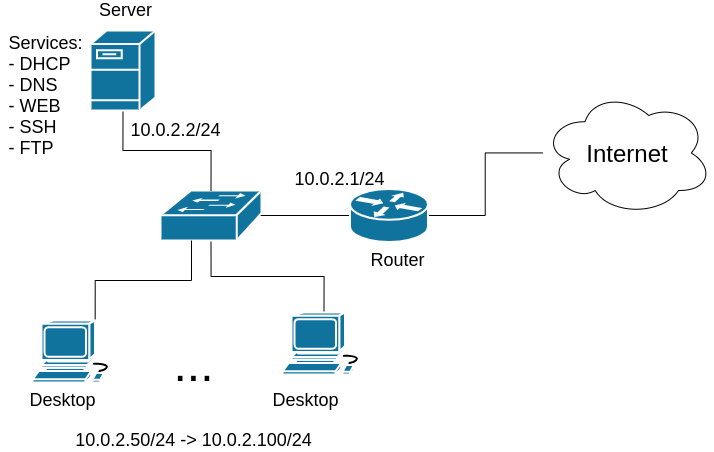
\includegraphics[width=\linewidth]{./imgs/Hinh-1.png}
  \caption{\bfseries Sơ đồ hệ thống mạng của công ty Tam Quốc}
\end{minipage}

\renewcommand{\arraystretch}{1.5}
\setcounter{subsection}{0}
\pagenumbering{arabic}
\phantomsection
\subsection{(10\%) Tạo và phân quyền cho thư mục /data}
\setcounter{figure}{0}

\newpage

\end{document}
